\documentclass[11pt]{article}

\usepackage[T1]{fontenc}
\usepackage[utf8]{inputenc}
\usepackage{lmodern}
\usepackage{microtype}
\usepackage[a4paper,margin=30mm]{geometry}
\usepackage{amsmath,amssymb,amsthm,mathtools}
\usepackage{booktabs}
\usepackage{array}
\usepackage{enumitem}
\usepackage{xcolor}
\usepackage{graphicx}
\usepackage{tikz}
\usetikzlibrary{arrows.meta,positioning,fit,calc,shapes.geometric}
\usepackage{listings}
\usepackage{url}
\usepackage[numbers,sort&compress]{natbib}
\usepackage{hyperref}
\usepackage[nameinlink,noabbrev]{cleveref}

\definecolor{deepblue}{RGB}{26,58,99}
\definecolor{deepgreen}{RGB}{22,103,72}
\definecolor{softgray}{RGB}{245,247,249}
\definecolor{codeblue}{RGB}{28,73,129}
\hypersetup{
  colorlinks=true,
  linkcolor=deepblue,
  citecolor=deepgreen,
  urlcolor=deepblue,
  pdfauthor={Lluis Eriksson},
  pdftitle={Marked Rooted-Tree Summation for Polymer Cluster Expansions with Holes: A Lean 4 Formalization},
  pdfsubject={Machine-checked rooted-tree and target-preserving polymer bounds},
  pdfkeywords={Lean 4, cluster expansion, polymer model, rooted tree, Ursell function, renormalization group}
}

\lstdefinelanguage{Lean}{
  morekeywords={theorem,def,noncomputable,namespace,end,by,exact,simpa,using,have,let,where,if,then,else,fun,forall,exists,open,import,structure,abbrev,variable},
  sensitive=true,
  morecomment=[l]{--},
  morecomment=[s]{/-}{-/},
  morestring=[b]"
}
\lstset{
  language=Lean,
  basicstyle=\ttfamily\small,
  keywordstyle=\color{codeblue}\bfseries,
  commentstyle=\color{deepgreen},
  backgroundcolor=\color{softgray},
  frame=single,
  rulecolor=\color{black!15},
  breaklines=true,
  columns=fullflexible,
  keepspaces=true,
  showstringspaces=false,
  xleftmargin=0.5em,
  xrightmargin=0.5em,
  aboveskip=0.8em,
  belowskip=0.8em
}

\newtheorem{theorem}{Theorem}[section]
\newtheorem{proposition}[theorem]{Proposition}
\newtheorem{lemma}[theorem]{Lemma}
\newtheorem{corollary}[theorem]{Corollary}
\newtheorem{definition}[theorem]{Definition}
\newtheorem{remark}[theorem]{Remark}
\newtheorem{assumption}[theorem]{Assumption}

\newcommand{\N}{\mathbb N}
\newcommand{\R}{\mathbb R}
\newcommand{\C}{\mathbb C}
\newcommand{\one}{\mathbf 1}
\newcommand{\dd}{\mathrm d}
\newcommand{\card}{\operatorname{card}}
\newcommand{\supp}{\operatorname{supp}}
\newcommand{\skel}{\operatorname{skel}}
\newcommand{\Tree}{\mathcal T}
\newcommand{\Poly}{\mathcal P}
\newcommand{\ExpW}{\mathsf E}
\newcommand{\Leaf}{\mathsf L}
\newcommand{\Mom}{\mathsf M}
\newcommand{\TargetTerm}{\mathsf T}
\newcommand{\MarkedSum}{\mathsf S}
\newcommand{\incomp}{\not\sim}

\title{\textbf{Marked Rooted-Tree Summation for Polymer Cluster Expansions with Holes}\\[0.4em]
\large A Lean 4 Formalization}
\author{Lluis Eriksson}
\date{June 2026}

\begin{document}
\maketitle

\begin{abstract}
We present a machine-checked finite mechanism for obtaining target-sensitive geometric bounds in a second Ursell expansion of a hard-core polymer gas with holes.  The difficulty is not merely to sum trees: the proof must preserve the exact target union long enough to extract modified-metric decay, while also preserving parent--child incompatibility data long enough to perform a local leaf recursion.  We formalize the resulting proof architecture in Lean~4.  Its principal ingredients are: a normalized bound on the aggregate child-factorial weight of rooted labelled spanning trees; a parent-normalized incompatibility kernel controlled by factorial metric moments; a marked-root, bottom-up fixed-tree summation; and a target-preserving composition theorem.  If $M$ denotes the geometric moment constant, the formalized marked-root estimate has the orderwise form
\[
  (n+1)\,\MarkedSum_n(r)\le M(4M^2)^n,
\]
and, after extracting target decay before enlarging the exact-union fiber,
\[
  \TargetTerm_n(Y)\le M\,e^{-\rho m(Y)}(4M^2)^n.
\]
The artifact pins the exact upstream commit, Lean toolchain, and Mathlib revision and exposes stable publication-facing theorem names.  The result is a finite combinatorial and geometric formalization; it does not prove the model-specific raw Yang--Mills activity estimate, a continuum limit, or a mass gap.
\end{abstract}

\paragraph{Keywords.}
Lean 4; cluster expansion; polymer model; Ursell function; rooted tree; modified metric; renormalization group; constructive field theory.

\paragraph{Artifact.}
The accompanying repository contains the manuscript, Lean companion, pinned dependency data, CI workflow, theorem map, and reproducibility instructions.  The exact upstream source state is commit
\texttt{83d18a113e3fa22ada23b13361fb84015a1c80ed} of \texttt{THE-ERIKSSON-PROGRAMME}.

\tableofcontents

\section{Introduction}

Cluster expansions convert logarithms of partition functions into sums over connected configurations.  Their conceptual statement is simple, but quantitative constructive applications require unusually strict information discipline.  In a polymer expansion with holes, two pieces of information are especially easy to lose:
\begin{enumerate}[label=(\roman*),leftmargin=2.5em]
  \item the \emph{exact target union} $Y$, which carries the geometric decay needed by the downstream renormalization-group estimate;
  \item the \emph{local tree structure}, which is needed to sum one child polymer through its incompatibility relation with its parent.
\end{enumerate}
If either is discarded prematurely, a finite sum remains, but the desired volume-uniform, target-dependent bound need not.

This paper isolates and formalizes a proof order that preserves both.  The exact target fiber is retained while a stitching inequality extracts a factor $e^{-\rho m(Y)}$.  Only then is a root cube $r\in\skel(Y)$ marked and the target fiber enlarged to a rooted overcount.  At fixed tree shape, nonroot variables are eliminated from the leaves inward.  A normalization by the parent metric cancels globally because every appearance of a vertex as a parent is counted by its rooted child count.  The remaining factorial degree weights are summed over labelled trees using a parent-profile argument.

The resulting formalized mechanism is summarized by
\begin{equation}\label{eq:main-pipeline}
\boxed{\begin{gathered}
\text{exact target fiber}\to\text{target decay}\to\text{marked root}\\
\to\text{local leaf recursion}\to 4^n\text{ closure}
\end{gathered}}
\end{equation}

The construction belongs to the classical lineage of tree-graph identities and abstract polymer expansions \citep{penrose1967,kotecky1986,fernandez2007,brydges1986}.  Its source-facing motivation is the with-holes renormalization-group organization in the Balaban--Dimock literature \citep{dimock2011,dimock2012,dimock2013}.  The contribution here is an end-to-end Lean~4 decomposition of a specific target-preserving leaf-summation mechanism, with explicit constants and a reproducible theorem map.  Lean~4 and Mathlib provide the proof environment \citep{demoura2021,mathlib2020}; the work also fits a broader recent effort to formalize mathematically structured quantum field theory \citep{douglas2026}.

\subsection{Why this is an ``infinity'' result only in a controlled sense}

The motivating language of ``marked infinities'' is not cardinal arithmetic.  It refers to a recurring analytic principle: when an infinite or eventually infinite expansion is approached through finite truncations, the physically relevant information is often a marker---a root, target, boundary condition, or direction of approach---that must survive until a uniform estimate has been extracted.  The present theorem is entirely finite at each order $n$.  Its purpose is to produce a geometric ratio that can later justify an infinite order sum.

\subsection{Contributions}

The formalized result has four publication-facing layers.
\begin{enumerate}[leftmargin=2.5em]
  \item A normalized aggregate bound for rooted child-factorial weights of complete-graph spanning trees:
  \begin{equation}\label{eq:four-bound-intro}
    \frac{n+1}{(n+1)!}
    \sum_{T\in\Tree_{n+1}}
    \prod_{v=0}^{n} c_T(v)!
    \le 4^n.
  \end{equation}
  \item A parent-normalized hard-core moment kernel whose local sums are factorially controlled.
  \item A marked-root fixed-tree recursion and its aggregate consequence
  \begin{equation}\label{eq:marked-intro}
    (n+1)\MarkedSum_n(r)\le M(4M^2)^n.
  \end{equation}
  \item A target-preserving composition theorem
  \begin{equation}\label{eq:target-intro}
    \TargetTerm_n(Y)\le M\,\ExpW_\rho(Y)(4M^2)^n,
  \end{equation}
  where $\ExpW_\rho(Y)=e^{-\rho m(Y)}$ in the source-facing specialization.
\end{enumerate}

The companion project exposes these layers as three short theorem names while retaining the full hypotheses of the verified upstream statements.

\subsection{Scope}

The formalization does not construct a concrete Yang--Mills fluctuation activity.  In particular, it does not prove the analytic estimate that would identify a physical activity with the abstract polymer weight entering the theorem.  It also does not prove a continuum limit, Osterwalder--Schrader reconstruction, or a continuum mass gap.  These exclusions are mathematical boundaries, not editorial caveats.

\section{Polymer systems with holes}

We record the finite structure abstracted by the Lean development.  The notation is chosen to expose the proof rather than reproduce every implementation type.

\subsection{Active skeleton and full target}

Let $\Lambda$ be a finite periodic lattice and let $\mathcal H$ be a finite family of hole regions.  A polymer $Q$ carries a full support $|Q|\subseteq\Lambda$ and an active skeleton
\[
  \skel_{\mathcal H}(Q)\subseteq |Q|.
\]
Hard-core incompatibility is determined by active intersection,
\[
  Q\incomp Q'
  \quad\Longleftrightarrow\quad
  \skel_{\mathcal H}(Q)\cap\skel_{\mathcal H}(Q')\ne\varnothing.
\]
The full support and active skeleton play different roles.  The skeleton controls connectivity and local incompatibility summation; the full union labels the target activity.

For a tuple $\mathbf Q=(Q_0,\dots,Q_n)$, write
\[
  U(\mathbf Q)=\bigcup_{i=0}^{n}|Q_i|.
\]
The exact target fiber over $Y$ is
\[
  \mathfrak F_n(Y)
  =\{\mathbf Q:U(\mathbf Q)=Y\}.
\]
The exact equality $U(\mathbf Q)=Y$ is the geometric information that must not be forgotten before target decay is extracted.

\subsection{Modified metric and shifted size}

Let $d_M(Q)$ denote the modified metric associated with the hole geometry, and define the strictly positive shifted size
\begin{equation}\label{eq:m-def}
  m(Q)=d_M(Q)+1.
\end{equation}
The corresponding exponential weight is
\begin{equation}\label{eq:exp-weight}
  \ExpW_\rho(Q)=e^{-\rho m(Q)}.
\end{equation}
The finite geometry provides a stitching inequality of the form
\begin{equation}\label{eq:stitch}
  m(Y)\le \sum_{i=0}^{n}m(Q_i)
  \qquad
  \text{whenever }U(\mathbf Q)=Y
  \text{ and the tuple is incompatibility-connected.}
\end{equation}
Consequently, for $\rho\ge0$,
\begin{equation}\label{eq:stitch-exp}
  \prod_{i=0}^{n}\ExpW_\rho(Q_i)
  \le \ExpW_\rho(Y).
\end{equation}

\subsection{Second Ursell tree term}

For a tuple $\mathbf Q$, let $G(\mathbf Q)$ be its incompatibility graph on $\{0,\dots,n\}$.  A nonnegative weighted tree term with exact target $Y$ has the schematic form
\begin{equation}\label{eq:target-tree-term}
  \TargetTerm_n^w(Y)
  =\frac{1}{(n+1)!}
  \sum_{\mathbf Q\in\mathfrak F_n(Y)}
  \sum_{T\in\Tree(G(\mathbf Q))}
  \prod_{i=0}^{n}w(Q_i).
\end{equation}
The formalized object uses the precise finite polymer carrier and spanning-tree predicate.  The nonnegative form is a majorant for the absolute Ursell coefficient after a tree-graph step.

\section{The rooted tree-profile bound}

The leaf recursion assigns a factorial cost to each rooted child count.  This section explains how those costs are summed over all labelled complete-graph spanning trees.

\subsection{Child-count profiles}

Root every tree $T$ on $\{0,\dots,n\}$ at $0$.  Let
\[
  c_T(v)=\#\{u:\operatorname{parent}_T(u)=v\}
\]
be the number of rooted children of $v$.  Then
\begin{equation}\label{eq:child-sum}
  \sum_{v=0}^{n}c_T(v)=n.
\end{equation}
The key weighted tree sum is
\[
  A_n=\sum_{T\in\Tree_{n+1}}\prod_{v=0}^{n}c_T(v)!.
\]

A direct Cayley count is not the proof used in the artifact.  Instead, the tree is injected into its parent map on the $n$ nonroot labels.  Parent maps are grouped by the profile
\[
  \mathbf c=(c(0),\dots,c(n)),
  \qquad c(v)\in\N,
  \qquad \sum_v c(v)=n.
\]
For a fixed profile, the product $\prod_v c(v)!$ pays for the permutations within the parent fibers.  The total fixed-profile cost is bounded by a single global $n!$ factor.  The number of weak compositions of $n$ into $n+1$ parts is
\begin{equation}\label{eq:profile-count}
  \binom{2n}{n}\le4^n.
\end{equation}
This gives $A_n\le n!4^n$.

\begin{theorem}[Normalized rooted child-factorial tree bound]\label{thm:tree-profile}
For every $n\in\N$,
\begin{equation}\label{eq:tree-profile-main}
  \frac{n+1}{(n+1)!}
  \sum_{T\in\Tree_{n+1}}
  \prod_{v=0}^{n}c_T(v)!
  \le4^n.
\end{equation}
\end{theorem}

\begin{proof}[Proof architecture]
The formal proof performs the following finite steps.
\begin{enumerate}[leftmargin=2.5em]
  \item Encode each rooted tree by the BFS parent map on the nonroot labels and prove injectivity on spanning trees.
  \item Partition parent maps by their child-count profile.
  \item For a fixed profile, encode a fiber family together with local permutations into a global permutation of $n$ labels.  This proves that the number of fiber families times $\prod_v c(v)!$ is at most $n!$.
  \item Count profiles by a finite antidiagonal, identify the count with $\binom{2n}{n}$, and use $\binom{2n}{n}\le4^n$.
  \item Cast the natural-number inequality to $\R$ and simplify
  \[
    \frac{n+1}{(n+1)!}\,n!=1.
  \]
\end{enumerate}
Every step is a theorem in the pinned Lean source; no asymptotic estimate is used.
\end{proof}

\begin{remark}[Central-binomial refinement]
The development also retains the sharper intermediate bound with $\binom{2n}{n}$ visible.  The published geometric closure uses $4^n$ because it composes transparently with the moment constant.  An exact Catalan improvement would require additional rooted plane-tree structure; it is not claimed here.
\end{remark}

\section{Parent-normalized moment kernels}

The tree-profile theorem controls shape entropy.  The analytic-geometric input controls the polymer assigned to each vertex.

\subsection{Hard-core moment kernel}

Fix $\kappa_0>0$.  For polymers $Q,Q'$ and a moment index $j\in\N$, define
\begin{equation}\label{eq:moment-kernel}
  K_j(Q,Q')
  =\one_{\{Q\incomp Q'\}}
    m(Q')^j\ExpW_{2\kappa_0}(Q').
\end{equation}
The hole geometry supplies a constant $M=M(d,\kappa_0)\ge1$ such that
\begin{equation}\label{eq:child-moment}
  \sum_{Q'}K_j(Q,Q')
  \le j!\,M^{j+1}\,m(Q).
\end{equation}
There is also a rooted version: for every active cube $r$,
\begin{equation}\label{eq:root-moment}
  \sum_{Q:\,r\in\skel(Q)}m(Q)^j\ExpW_{2\kappa_0}(Q)
  \le j!\,M^{j+1}.
\end{equation}
The exact Lean theorem derives these from finite modified-metric summability under explicit hole-disjointness, no-inter-hole-edge, nonempty-hole, and numerical entropy hypotheses.

\subsection{Why normalization by the parent metric is necessary}

The right-hand side of \cref{eq:child-moment} depends on the parent $Q$ through $m(Q)$.  A uniform tree-walk lemma cannot consume it directly.  The formal proof divides each nonroot edge factor by the parent metric:
\begin{equation}\label{eq:normalized-kernel}
  \widetilde K_j(Q,Q')
  =\frac{m(Q')^jK_0(Q,Q')}{m(Q)}.
\end{equation}
Since $m(Q)>0$, \cref{eq:child-moment} implies
\begin{equation}\label{eq:normalized-budget}
  \sum_{Q'}\widetilde K_j(Q,Q')
  \le j!\,M^{j+1}.
\end{equation}

This division is not cosmetic.  It is the algebraic move that converts a parent-dependent budget into a local constant while retaining the incompatibility edge.

\subsection{Global cancellation of parent metrics}

For a fixed rooted tree $T$ and assignment $X:v\mapsto Q_v$, let $p_T(v)$ be the parent of nonroot $v$.  Then
\begin{equation}\label{eq:parent-product}
  \prod_{v\ne0}m(Q_{p_T(v)})
  =\prod_{a=0}^{n}m(Q_a)^{c_T(a)}.
\end{equation}
The denominators introduced in \cref{eq:normalized-kernel} therefore cancel exactly against the metric moments assigned to the vertices.  In Lean, this is proved from the partition of nonroot vertices into rooted child fibers, not by informal multiplicity reasoning.

\section{Fixed-tree leaf elimination}

We now combine the normalized budgets along one tree.

\subsection{Vertexwise tree walk}

A generic finite theorem eliminates variables from maximal depth toward the root.  Each nonroot vertex $v$ has a budget $A(v)$ satisfying
\[
  \sum_y I_v(x,y)\le A(v),
\]
while the root carries a pinned weight.  The theorem concludes
\begin{equation}\label{eq:vertex-walk}
  \sum_X
  \left(\prod_{v\ne0}I_v(X_{p(v)},X_v)\right)
  w_0(X_0)
  \le
  \left(\prod_{v\ne0}A(v)\right)
  \sum_y w_0(y).
\end{equation}
The proof is an induction that removes a maximal-level leaf and reindexes the remaining assignments.  The vertex-dependent form matters: the budget at $v$ depends on $c_T(v)$.

\subsection{Fixed-tree bound}

For a fixed tree $T$, set
\[
  A(v)=c_T(v)!\,M^{c_T(v)+1}.
\]
The normalized child estimate \cref{eq:normalized-budget} supplies $A(v)$ for every nonroot vertex.  The rooted moment estimate \cref{eq:root-moment} supplies the same factorial-moment factor at the root.  Therefore
\begin{proposition}[Fixed-tree marked-root estimate]\label{prop:fixed-tree}
For every fixed complete-graph spanning tree $T$,
\begin{equation}\label{eq:fixed-tree}
  \mathsf F_T(r)
  \le
  \left(\prod_{v=0}^{n}c_T(v)!\right)
  M^{2n+1}.
\end{equation}
\end{proposition}

\begin{proof}[Exponent audit]
Every vertex contributes $M^{c_T(v)+1}$.  Using \cref{eq:child-sum},
\[
  \sum_{v=0}^{n}(c_T(v)+1)=n+(n+1)=2n+1.
\]
Hence the total moment power is exactly $M^{2n+1}$.  The formal proof separately establishes the factorial product, power product, and exponent sum before recombining them.
\end{proof}

\section{Marked-root geometric closure}

\subsection{The marked-root sum}

Let $\MarkedSum_n(r)$ be the normalized nonnegative tree sum in which coordinate $0$ is constrained by $r\in\skel(Q_0)$.  Marking one coordinate of an $(n+1)$-tuple creates an outer factor $n+1$.  The Ursell normalization contributes $(n+1)!^{-1}$.  This is precisely the normalization in \cref{thm:tree-profile}.

\begin{theorem}[Marked-root leaf summation]\label{thm:marked-root}
Under the explicit hole-geometry and metric-summability hypotheses of the Lean statement,
\begin{equation}\label{eq:marked-root-main}
  (n+1)\MarkedSum_n(r)
  \le M\,(4M^2)^n.
\end{equation}
\end{theorem}

\begin{proof}[Assembly]
The raw incompatibility-tree sum is first bounded by a sum over complete-graph tree shapes that retains a hard-core indicator on each BFS parent edge.  The vertex weights are then dominated by the spare exponential weight entering the moment kernel.  Applying \cref{prop:fixed-tree} and summing shapes gives
\[
  (n+1)\MarkedSum_n(r)
  \le
  \frac{n+1}{(n+1)!}
  M^{2n+1}
  \sum_T\prod_vc_T(v)!.
\]
Theorem~\ref{thm:tree-profile} yields
\[
  (n+1)\MarkedSum_n(r)
  \le M^{2n+1}4^n
  =M(4M^2)^n.
\]
The Lean theorem names the closed leaf ratio
\begin{equation}\label{eq:leaf-constant}
  L(d,\kappa_0)=4M(d,\kappa_0)^2.
\end{equation}
\end{proof}

\begin{figure}[t]
\centering
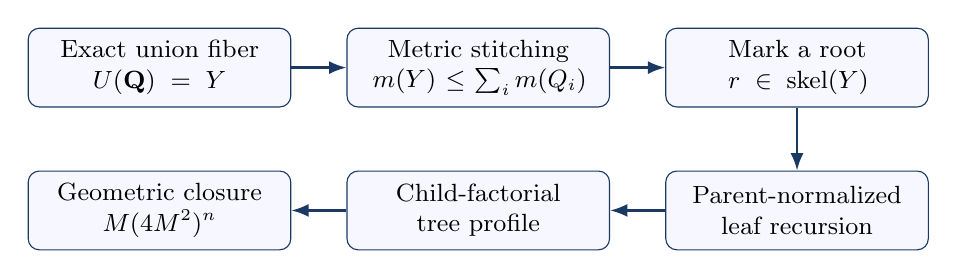
\begin{tikzpicture}[
  node distance=8mm and 7mm,
  box/.style={draw=deepblue,rounded corners,fill=blue!3,align=center,minimum height=10mm,text width=31mm,font=\small},
  arr/.style={-{Latex[length=2.2mm]},thick,deepblue}
]
\node[box] (fiber) {Exact union fiber\\$U(\mathbf Q)=Y$};
\node[box,right=of fiber] (stitch) {Metric stitching\\$m(Y)\le\sum_i m(Q_i)$};
\node[box,right=of stitch] (root) {Mark a root\\$r\in\skel(Y)$};
\node[box,below=of root] (walk) {Parent-normalized\\leaf recursion};
\node[box,left=of walk] (shape) {Child-factorial\\tree profile};
\node[box,left=of shape] (close) {Geometric closure\\$M(4M^2)^n$};
\draw[arr] (fiber) -- (stitch);
\draw[arr] (stitch) -- (root);
\draw[arr] (root) -- (walk);
\draw[arr] (walk) -- (shape);
\draw[arr] (shape) -- (close);
\end{tikzpicture}
\caption{The proof order.  The exact target is used before the marked-root enlargement; the tree edges are retained until the child variables have been locally summed.}
\label{fig:pipeline}
\end{figure}

\section{Target-preserving decay}

The marked-root theorem is not yet target-sensitive: $Y$ has disappeared.  The target-preserving composition theorem ensures that it disappears only after paying for its decay.

\subsection{Weight splitting}

Let $w,u\ge0$ be weights satisfying
\begin{equation}\label{eq:split}
  w(Q)\le \ExpW_\rho(Q)\,u(Q),
  \qquad \rho\ge0.
\end{equation}
For each tuple in the exact target fiber, \cref{eq:stitch-exp} gives
\[
  \prod_{i=0}^{n}w(Q_i)
  \le
  \ExpW_\rho(Y)\prod_{i=0}^{n}u(Q_i).
\]
Thus
\begin{equation}\label{eq:target-extract}
  \TargetTerm_n^w(Y)
  \le
  \ExpW_\rho(Y)\,\TargetTerm_n^u(Y).
\end{equation}
Only now do we choose $r\in\skel(Y)$ and enlarge the exact target fiber to the marked-root sum.

\begin{theorem}[Target-preserving weighted-tree bound]\label{thm:target}
Assume \cref{eq:split}, assume $u(Q)\le\ExpW_{2\kappa_0}(Q)$, and assume $r\in\skel(Y)$.  Under the finite hole-geometry hypotheses,
\begin{equation}\label{eq:target-main}
  \TargetTerm_n^w(Y)
  \le
  M\,\ExpW_\rho(Y)\,(4M^2)^n.
\end{equation}
\end{theorem}

\begin{proof}
Equation~\eqref{eq:target-extract} extracts the target factor.  The fixed-union term for $u$ is at most $(n+1)\MarkedSum_n(r)$ because every tuple with union $Y$ contains the marked cube in at least one coordinate, and a coordinate permutation moves it to position $0$.  Theorem~\ref{thm:marked-root} closes the remaining sum.
\end{proof}

\begin{remark}[The forbidden proof order]\label{rem:forbidden-order}
If one first replaces the exact-union fiber by a global marked-root sum, the resulting object no longer contains $Y$.  A bound with $e^{-\rho m(Y)}$ cannot then be derived from that object alone.  Reintroducing target decay as a hypothesis would be circular.  This failure mode is encoded in the theorem architecture: target extraction and leaf summation are separate theorems, and the former is applied first.
\end{remark}

\subsection{Geometric order sum}

Suppose a model-specific activity estimate contributes a factor $\varepsilon^{n+1}$ at order $n$.  Then \cref{thm:target} yields
\[
  \varepsilon^{n+1}\TargetTerm_n^w(Y)
  \le
  M\varepsilon\,\ExpW_\rho(Y)
  (4M^2\varepsilon)^n.
\]
Hence the following consequence is immediate.

\begin{corollary}[Closed geometric majorant]\label{cor:geometric}
If $4M^2\varepsilon<1$, then
\begin{equation}\label{eq:closed-majorant}
  \sum_{n=0}^{\infty}
  \varepsilon^{n+1}\TargetTerm_n^w(Y)
  \le
  \frac{M\varepsilon}{1-4M^2\varepsilon}
  \ExpW_\rho(Y).
\end{equation}
\end{corollary}

The corollary is a standard geometric-series calculation.  The formal contribution of the present work is the finite orderwise input with the correct target factor and an explicit ratio.

\section{Lean formalization}

\subsection{Pinned environment}

The artifact is a small publication companion around a pinned, larger formalization repository.  Its locked environment is shown in \cref{tab:versions}.

\begin{table}[h]
\centering
\caption{Pinned software and source state.}
\label{tab:versions}
\begin{tabular}{@{}ll@{}}
\toprule
Component & Locked value \\
\midrule
Lean & \texttt{leanprover/lean4:v4.29.0-rc6} \\
Mathlib & \texttt{07642720480157414db592fa85b626dafb71355b} \\
Upstream repository & \texttt{lluiseriksson/THE-ERIKSSON-PROGRAMME} \\
Upstream commit & \texttt{83d18a113e3fa22ada23b13361fb84015a1c80ed} \\
Rooted-tree source blob & \texttt{1415686403c26536da8736a9021237773c7467dc} \\
Appendix-F source blob & \texttt{0307d11b95d4385d4ea39067290e7eec929cd7f6} \\
\bottomrule
\end{tabular}
\end{table}

The companion module gives stable, paper-facing names to three upstream theorems.  It adds no axiom and no opaque mathematical field.

\subsection{Publication-facing endpoints}

The first endpoint is an exact alias of \cref{thm:tree-profile}.

\begin{lstlisting}[caption={The normalized rooted child-factorial bound.}]
theorem normalizedRootedChildFactorialTreeBound (n : Nat) :
    ((n : Real) + 1) *
        (((n + 1).factorial : Real))^-1 *
        (sum T in spanningTrees (top : SimpleGraph (Fin (n + 1))),
          prod v : Fin (n + 1),
            ((rootedChildCount T v).factorial : Real))
      <= (4 : Real)^n
\end{lstlisting}

The marked-root endpoint retains every finite geometric hypothesis of \cref{thm:marked-root}; in particular, the hole conditions and the numerical summability condition are visible.  The target endpoint similarly exposes $w$, $u$, the split inequality, the target root, and the residual rate.

\begin{lstlisting}[caption={The target-preserving endpoint, abbreviated.}]
theorem targetPreservingWeightedTreeBound
    ...
    (hsplit : forall Q,
      w Q <= appendixFHoleExpWeight HF rate Q.val * u Q)
    (hu_exp : forall Q,
      u Q <= appendixFHoleExpWeight HF (2 * kappa0) Q.val)
    (hr : r in skeleton HF Y)
    ... :
    appendixFHoleHsharpWeightedTreeTerm HF zK w Y n <=
      appendixFSecondUrsellMomentConstant d kappa0 *
        appendixFHoleExpWeight HF rate Y *
        appendixFSecondUrsellLeafConstant d kappa0 ^ n
\end{lstlisting}

\subsection{Theorem dependency map}

The machine-checked dependency ladder is
\begin{equation}\label{eq:dependency-ladder}
\begin{gathered}
\text{parent-map fibers}\to\text{fixed-profile factorial budget}\\
\to\text{central-binomial profile count}\to\text{normalized }4^n\text{ bound}\\
\to\text{parent-product cancellation}\to\text{normalized child kernel}\\
\to\text{vertexwise tree walk}\to\text{fixed-tree moment bound}\\
\to\text{marked-root geometric bound}\to\text{target extraction}\\
\to\text{target-preserving orderwise bound}.
\end{gathered}
\end{equation}
The repository's \texttt{docs/THEOREM\_MAP.md} gives a one-line map from each paper theorem to the exact upstream theorem and file.

\subsection{Proof trust and oracle}

The build target compiles the companion module and then invokes Lean on an oracle file containing \texttt{\#print axioms} for the public endpoints.  The expected output is limited to standard classical principles inherited from Mathlib and the pinned core, normally
\[
  [\texttt{propext},\ \texttt{Classical.choice},\ \texttt{Quot.sound}].
\]
Static checks reject \texttt{sorry}, \texttt{admit}, and project-local \texttt{axiom} declarations in the companion source.  The CI workflow separately builds the paper and uploads the PDF.

\section{Mathematical interpretation}

\subsection{Entropy versus decay}

The proof makes a standard constructive competition explicit:
\[
  \text{configuration entropy}
  \quad\text{versus}\quad
  \text{local exponential decay}.
\]
The factor $4^n$ is a finite upper bound on rooted child-profile entropy.  The factor $M^{2n+1}$ is the cost of local metric moments.  Their product gives the leaf ratio $4M^2$ per extra vertex.  A model-specific activity amplitude $\varepsilon$ must then satisfy
\[
  4M^2\varepsilon<1.
\]
No cardinal hierarchy is involved; ``larger infinity'' is not the relevant concept.  What matters is whether an infinite order sum is dominated by a geometric series uniformly in the finite volume and target.

\subsection{The marker as conserved information}

The root and target have complementary roles.
\begin{itemize}[leftmargin=2em]
  \item The target $Y$ records \emph{where the final activity lives}.  It is conserved until its modified-metric decay has been extracted.
  \item The root $r$ records \emph{where the local summation is pinned}.  It converts global configuration entropy into a rooted local budget.
\end{itemize}
This can be viewed as a finite analogue of compactifying a limit while remembering the direction of approach: the boundary object alone is not enough; the marker carries the observable information.

\subsection{Why the theorem is reusable}

The finite tree-profile layer is independent of holes and polymer geometry.  The fixed-tree walk layer is independent of the particular modified metric once supplied with local child and root budgets.  The with-holes specialization enters only through:
\begin{enumerate}[label=(\alph*),leftmargin=2.5em]
  \item the incompatibility relation;
  \item the metric moment estimates;
  \item the stitching inequality;
  \item the nonempty active skeleton used to choose the root.
\end{enumerate}
This factorization of concerns is useful both mathematically and formally: alternative polymer geometries can reuse the tree engine without pretending that their analytic constants are identical.

\section{Related work and novelty boundary}

Tree-graph identities and polymer expansions have a long history \citep{penrose1967,brydges1986,kotecky1986,fernandez2007}.  Degree profiles, weak compositions, and central binomial estimates are classical enumerative tools \citep{stanley2012,flajolet2009}.  The Balaban--Dimock program supplies the source-facing context in which connected polymers with holes, modified metrics, and repeated cluster expansions occur \citep{dimock2011,dimock2012,dimock2013}.

The formalization does not claim a new classical tree-graph identity.  Its contribution is the machine-checked assembly of a particular proof pipeline in which several superficially harmless reorderings are invalid for the target-sensitive conclusion.  In particular:
\begin{itemize}[leftmargin=2em]
  \item the target is not replaced by a global sum before target decay is extracted;
  \item the tree is not replaced by independent vertex weights before parent--child moment summation;
  \item the parent-dependent moment factor is normalized and canceled exactly rather than bounded globally;
  \item the $(n+1)$ marking factor is canceled by the Ursell normalization and the rooted tree-profile estimate, not absorbed into an unspecified constant.
\end{itemize}

To the best of our knowledge, no prior Lean artifact formalizes this exact target-preserving with-holes second-Ursell leaf-summation pipeline.  This is a scoped literature statement, not a claim of priority over all formal or informal cluster-expansion arguments.

\section{Limitations and open obligations}

The theorem begins after a polymer weight has already been constructed.  A physical application to four-dimensional lattice Yang--Mills would additionally require a model-specific chain such as
\[
\begin{gathered}
\text{gauge-fixed Hessian}\to\text{coercive precision}\to\text{localized covariance}\\
\to\text{fluctuation integral}\to\text{raw local activity}\to\text{source weight split}.
\end{gathered}
\]
None of those identifications follows from the finite theorem.  In the present source-facing architecture, the remaining analytic obligations include:
\begin{enumerate}[leftmargin=2.5em]
  \item an exact definition of the raw activity from the physical RG integral;
  \item a pointwise or normed activity estimate with modified-metric decay;
  \item the precise source-to-formal translation of constants and supports;
  \item integrability and measure-identification statements;
  \item the numerical smallness $4M^2\varepsilon<1$ in the physical parameter window.
\end{enumerate}
Even discharging these would not by itself construct the continuum theory.  Thermodynamic and continuum limits, reflection positivity, reconstruction, nontriviality, and a continuum spectral gap remain separate problems.

\section{Reproducibility}

A clean build is intended to require Git, a POSIX shell, and \texttt{elan}.  From the repository root:
\begin{lstlisting}[language=bash]
lake update
lake build MarkedRootedClosure
lake env lean MarkedRootedClosure/Oracle.lean
make -C paper clean all
bash scripts/check_no_placeholders.sh
python3 scripts/check_artifact.py
\end{lstlisting}
The first command fetches the exact pinned upstream project and its pinned Mathlib revision.  The repository also includes a GitHub Actions workflow with separate Lean and paper jobs, machine-readable lock data, citation metadata, a release script, and an artifact-evaluation guide.

For long-term archival, the recommended process is: tag an immutable release; attach the exact source ZIP and PDF; archive the release on Zenodo or an institutional service; add the resulting DOI to \texttt{CITATION.cff}; and record the final CI URL and release hash in the submitted manuscript.

\section{Conclusion}

The formal result can be summarized in one sentence: \emph{extract target decay while the exact union is still present, then mark a root and sum the remaining tree locally}.  That proof order produces the explicit finite bound
\[
  \TargetTerm_n(Y)
  \le
  M\,e^{-\rho m(Y)}(4M^2)^n,
\]
with every combinatorial and geometric factor exposed.  Lean~4 verifies the parent-profile count, metric cancellation, leaf recursion, root moment, tree sum, and target composition as separate reusable theorems.

The artifact is deliberately narrower than the larger constructive field-theory programme that motivated it.  That narrowness is a strength: the statement can be audited, rebuilt, cited, and reused without confusing a finite cluster-expansion theorem with the still-open model-specific and continuum analysis.

\appendix

\section{Public theorem signatures}\label{app:signatures}

The following are the full public theorem names exposed by the companion:
\begin{lstlisting}
MarkedRootedClosure.normalizedRootedChildFactorialTreeBound
MarkedRootedClosure.markedRootLeafGeometricBound
MarkedRootedClosure.targetPreservingWeightedTreeBound
\end{lstlisting}
Their bodies are exact applications of the pinned upstream endpoints:
\begin{lstlisting}
YangMills.KP.rootedChildCount_factorialTreeSum_normalized_le_four_pow
YangMills.RG.appendixFHoleHsharpWeightedTreeMarkedRootSum_le_geometric_of_expWeight
YangMills.RG.appendixFHoleHsharpWeightedTreeTerm_le_geometric_of_expWeight_leafSummation
\end{lstlisting}
The full Lean signatures, including all geometry hypotheses, are contained in the companion source file \texttt{PaperTheorems.lean}.

\section{Constant audit}\label{app:constants}

Let
\[
  M=\texttt{appendixFSecondUrsellMomentConstant}(d,\kappa_0),
\]
which is nonnegative in the formal development, and define
\[
  L=\texttt{appendixFSecondUrsellLeafConstant}(d,\kappa_0)=4M^2.
\]
For a fixed tree with $n+1$ vertices, the root and child moment exponents sum to $2n+1$, producing $M^{2n+1}$.  The normalized shape sum contributes at most $4^n$, so
\[
  M^{2n+1}4^n=M(4M^2)^n=ML^n.
\]
There is no hidden order-dependent constant.  The later geometric series has ratio $L\varepsilon$.

\section{Reviewer checklist}\label{app:review}

A reviewer can audit the central claim in the following order:
\begin{enumerate}[leftmargin=2.5em]
  \item Check \texttt{archive/UPSTREAM.lock} and the exact dependency SHA in \texttt{lakefile.lean}.
  \item Inspect the three wrapper statements in \texttt{PaperTheorems.lean}.
  \item Build \texttt{MarkedRootedClosure} and run the oracle file.
  \item Inspect the upstream implementations listed in \texttt{docs/THEOREM\_MAP.md}.
  \item Compare \cref{thm:tree-profile,thm:marked-root,thm:target} with the compiled signatures.
  \item Confirm that the limitations paragraph remains unchanged in the abstract and conclusion.
\end{enumerate}

\begin{thebibliography}{99}

\bibitem[Penrose(1967)]{penrose1967}
O. Penrose.
\newblock Convergence of fugacity expansions for classical systems.
\newblock In T. A. Bak, editor, \emph{Statistical Mechanics: Foundations and Applications}, pages 101--109. W. A. Benjamin, 1967.

\bibitem[Koteck\'y and Preiss(1986)]{kotecky1986}
R. Koteck\'y and D. Preiss.
\newblock Cluster expansion for abstract polymer models.
\newblock \emph{Communications in Mathematical Physics}, 103(3):491--498, 1986.

\bibitem[Fern\'andez and Procacci(2007)]{fernandez2007}
R. Fern\'andez and A. Procacci.
\newblock Cluster expansion for abstract polymer models: new bounds from an old approach.
\newblock \emph{Communications in Mathematical Physics}, 274(1):123--140, 2007.

\bibitem[Brydges(1986)]{brydges1986}
D. C. Brydges.
\newblock A short course on cluster expansions.
\newblock In K. Osterwalder and R. Stora, editors, \emph{Critical Phenomena, Random Systems, Gauge Theories}, pages 129--183. North-Holland, 1986.

\bibitem[Dimock(2013a)]{dimock2011}
J. Dimock.
\newblock The renormalization group according to Balaban---I. Small fields.
\newblock \emph{Reviews in Mathematical Physics}, 25(7):1330010, 2013. arXiv:1108.1335.

\bibitem[Dimock(2013b)]{dimock2012}
J. Dimock.
\newblock The renormalization group according to Balaban---II. Large fields.
\newblock \emph{Journal of Mathematical Physics}, 54(9):092301, 2013. arXiv:1212.5562.

\bibitem[Dimock(2014)]{dimock2013}
J. Dimock.
\newblock The renormalization group according to Balaban---III. Convergence.
\newblock \emph{Annales Henri Poincar\'e}, 15:2133--2170, 2014. arXiv:1304.0705.

\bibitem[de Moura and Ullrich(2021)]{demoura2021}
L. de Moura and S. Ullrich.
\newblock The Lean 4 theorem prover and programming language.
\newblock In \emph{Automated Deduction---CADE 28}, LNCS 12699, pages 625--635. Springer, 2021.

\bibitem[The mathlib Community(2020)]{mathlib2020}
The mathlib Community.
\newblock The Lean mathematical library.
\newblock In \emph{Proceedings of CPP 2020}, pages 367--381. ACM, 2020.

\bibitem[Douglas et al.(2026)]{douglas2026}
M. R. Douglas et al.
\newblock Formalization of quantum field theory.
\newblock arXiv:2603.15770, 2026.

\bibitem[Flajolet and Sedgewick(2009)]{flajolet2009}
P. Flajolet and R. Sedgewick.
\newblock \emph{Analytic Combinatorics}.
\newblock Cambridge University Press, 2009.

\bibitem[Stanley(2012)]{stanley2012}
R. P. Stanley.
\newblock \emph{Enumerative Combinatorics, Volume 1}, second edition.
\newblock Cambridge University Press, 2012.

\bibitem[Eriksson(2026)]{erikssonartifact2026}
L. Eriksson.
\newblock THE-ERIKSSON-PROGRAMME: machine-checked polymer and renormalization-group infrastructure.
\newblock Git repository, commit \texttt{83d18a113e3fa22ada23b13361fb84015a1c80ed}, 2026.

\end{thebibliography}

\end{document}
